% Supplement to the revised manuscript JCOMP-D-26-00768
% "Neural Pushforward Sampler for Transient Multi-modal and Singular Distributions
%  from Fokker--Planck Equations with Adversarial Training"
% Three steady-state examples removed from the revised manuscript for reasons of length.
\documentclass[11pt,a4paper]{article}
\usepackage[utf8]{inputenc}
\usepackage[T1]{fontenc}
\usepackage{lmodern}
\usepackage[margin=1in]{geometry}
\usepackage{amsmath,amssymb,amsfonts}
\usepackage{graphicx}
\usepackage{subcaption}
\usepackage{float}
\usepackage{placeins}
\usepackage{xcolor}
\usepackage[colorlinks=true,linkcolor=blue!60!black,urlcolor=blue!60!black]{hyperref}
\renewcommand{\mathbf}[1]{\boldsymbol{#1}}

% Colors marking the changes made in response to the referee reports (same as in the manuscript)
\definecolor{revtwocolor}{RGB}{200,90,0}    % Reviewer #2
\definecolor{revthreecolor}{RGB}{0,140,70}  % Reviewer #3
\newcommand{\revtwo}[1]{\textcolor{revtwocolor}{#1}}
\newcommand{\revthree}[1]{\textcolor{revthreecolor}{#1}}

\title{\vspace{-1.2cm}Supplement: three steady-state examples removed from the revised manuscript\\[4pt]
\large\itshape Neural Pushforward Sampler for Transient Multimodal and Singular Distributions from\\
Fokker--Planck Equations with Adversarial Training (JCOMP-D-26-00768)}
\author{Andrew Qing He \and Wei Cai}
\date{}

\begin{document}
\maketitle
\vspace{-1cm}

\section*{About this supplement}

The three examples below formed Sections~4.1--4.3 of the original submission (a one-dimensional
steady Ornstein--Uhlenbeck problem, and symmetric double-well potentials in one and two
dimensions). All three were re-run in response to the referee reports (adversarial training of
the test functions, comment~1 of Reviewer~\#2; $\sigma$-annealing and the two-group optimizer or
the mixed test-function bank, comment~4 of Reviewer~\#1, comment~3 of Reviewer~\#2 and comments~4,
5 and minor comment~4 of Reviewer~\#3). To stay within the page limit of the journal they were
then removed from the revised manuscript, which now opens its numerical section with the new
examples requested by the reviewers. The text below is reproduced as it stood in the revised
manuscript immediately before the removal; the colored passages mark the changes made in response
to Reviewer~\#2 (\revtwo{orange}) and Reviewer~\#3 (\revthree{green}). References to equations
and sections of the manuscript are written in words.

The source code and the results of the three examples are in this repository:
\begin{center}
\begin{tabular}{ll}
\S\ref{sup:ou} & \texttt{supplementary\_experiments/R2\_1\_adversarial\_sec41/}\\
\S\ref{sup:dp1d} & \texttt{supplementary\_experiments/R3\_M5\_optimizer\_comparison/}\\
\S\ref{sup:dp2d} & \texttt{supplementary\_experiments/R3\_m4\_double\_peak\_2d/}
\end{tabular}
\end{center}

\section{A one-dimensional steady-state problem}\label{sup:ou}

We first apply the method to a one-dimensional problem with a known analytical solution.

\subsection{Problem specification}
We consider the steady-state Fokker--Planck equation of \S2 of the manuscript on $\mathbb{R}$ with dimension $n=1$, drift coefficient $b(x) = -\theta (x - \mu)$, and diffusion coefficient $a(x) = \sigma^2$ where $\sigma$ is a constant.
The corresponding PDE is therefore:
\begin{equation} \label{eq:1d_fpe}
-\frac{\sigma^2}{2} \frac{\partial ^{2} \rho}{\partial x^{2}} + \frac{\partial }{\partial x}\left[ (-\theta (x-\mu)) \rho\right] = 0.
\end{equation}
For this test, we set $\sigma = \sqrt{2}$, $\theta = 1$, and $\mu = 2$. The analytical solution is the Gaussian distribution $\mathcal{N}(\mu, \sigma^2/2\theta) = \mathcal{N}(2, 1)$, with mean $\mu_{\text{true}} = 2$ and standard deviation $\sigma_{\text{true}} = 1$.

\subsection{Training configuration}
The neural pushforward mapping $F_{{\boldsymbol{\vartheta}}}$ was implemented as a network with architecture $(1, 10, 10, 1)$ and Tanh activation functions. The base distribution $\pi_{\text{base}}$ is the uniform distribution on $[0, 1]$.

The adversarial test functions were parameterized as $f^{(k)}(x) = \sin(w^{(k)} x + b^{(k)})$. A collection of $K=100$ such test functions was constructed. \revtwo{As in all the other examples, the parameters $\eta = \{w^{(k)}, b^{(k)}\}$ are trained adversarially. They are initialized by sampling $w^{(k)} \sim \mathcal{N}(0, 1.5^2)$ and $b^{(k)} \sim \mathcal{U}(0, 2\pi)$, and are then updated by gradient \emph{ascent} on the loss.} The batch size was set to $M=1{,}000$ samples.

\revtwo{The model was trained for 10,000 epochs by alternating between the two players. The generator parameters ${\boldsymbol{\vartheta}}$ of $F_{{\boldsymbol{\vartheta}}}$ minimize the loss function ${L}_{\text{total}}$ (defined in \S2.3 of the manuscript) using the Adam optimizer with an initial learning rate of $10^{-2}$, decayed linearly to $10^{-5}$ over the course of training. The test-function parameters $\eta$ maximize ${L}_{\text{total}}$ using SGD with learning rate $10^{-2}$, performing 5 ascent steps every 10 epochs and a single ascent step in the remaining epochs.}

\subsection{Results and performance}
\begin{figure}[htb]
    \centering
    \begin{subfigure}[t]{0.45\textwidth}
        \centering
        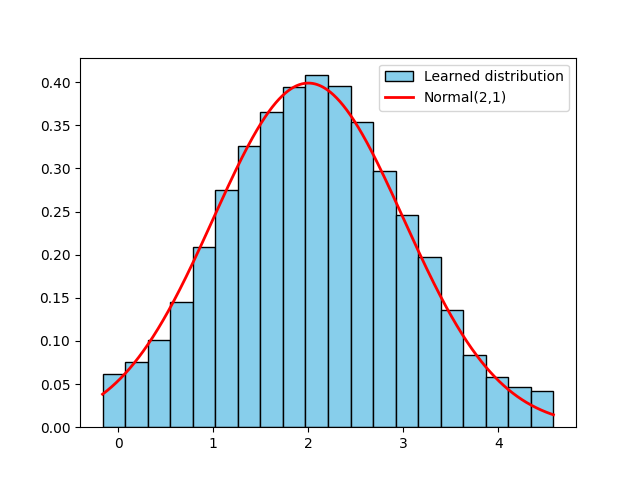
\includegraphics[width=\textwidth]{imgs/1dst_N21_adv_dist.png}
        \caption{Comparison of the learned and true probability density functions.}
    \end{subfigure}
    \hspace{1.5em}
    \begin{subfigure}[t]{0.45\textwidth}
        \centering
        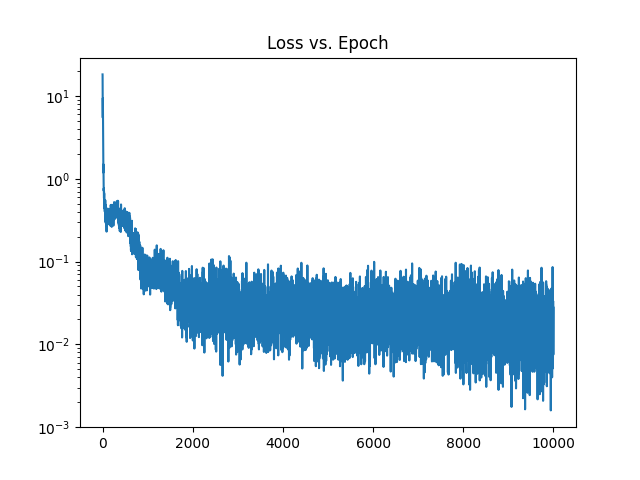
\includegraphics[width=\textwidth]{imgs/1dst_N21_adv_LvE.png}
        \caption{The convergence of the loss function over training steps (epochs).}
    \end{subfigure}
    \caption{Numerical results for the one-dimensional Fokker--Planck equation. (a) The pushforward network $F_{{\boldsymbol{\vartheta}}}$ learns to transform a uniform distribution into the target Gaussian distribution $\mathcal{N}(2,1)$, as the learned PDF shows \revtwo{good} agreement with the analytical solution. \revtwo{(b) Training loss ${L}_{\text{total}}$ (generator loss evaluated against the current adversarial test functions). After a rapid initial decrease, the loss fluctuates around $10^{-2}$, which is characteristic of the alternating min-max updates.}}
    \label{fig:1d_result}
\end{figure}

\revtwo{The training converged, with the loss decreasing from an initial value of $18.2$ to $2.8\times 10^{-2}$ at the end of training (with fluctuations of about an order of magnitude due to the adversarial updates). Figure~\ref{fig:1d_result}(a) shows close agreement between the learned and analytical PDFs. The empirical mean and standard deviation of the learned distribution are $\mu_{\text{learned}} = 2.0697$ and $\sigma_{\text{learned}} = 0.9542$, compared with the true values $\mu_{\text{true}}=2$ and $\sigma_{\text{true}}=1$, i.e., relative errors of $3.5\%$ and $4.6\%$, respectively. The figure shows a single run; over five independent random seeds, the learned mean lies in $[1.90, 2.14]$ and the learned standard deviation in $[0.84, 0.98]$. For comparison, when the test functions are kept frozen at their random initialization, the same generator achieves similar accuracy (mean $1.95 \pm 0.04$, standard deviation $0.94 \pm 0.02$ over five seeds). Thus, for this simple unimodal problem the adversarial updates neither help nor hurt noticeably.}

\FloatBarrier
\section{A one-dimensional double-peak distribution}\label{sup:dp1d}

We apply the method to a bimodal distribution arising from a double-well potential, as a first test of the framework on a multimodal probability distribution.

\subsection{Problem specification}
We consider a steady-state Fokker--Planck equation with a double-well potential $V(x) = (x^2 - 1)^2$, which creates two symmetric minima at $x = \pm 1$. The corresponding drift and diffusion coefficients are as follows: the problem is one-dimensional ($n=1$), with drift coefficient $b(x) = -\frac{\mathrm{d}V}{\mathrm{d}x} = -4x^3 + 4x = -4x(x^2 - 1)$ and constant diffusion coefficient $a(x) = \sigma^2$.

For this experiment, we set $\sigma = 0.6$. The resulting Fokker--Planck equation is:
\begin{equation}
-\frac{\sigma^2}{2} \frac{\partial^2 \rho}{\partial x^2} + \frac{\partial}{\partial x}[(-4x^3 + 4x) \rho] = 0.
\end{equation}

The steady-state solution corresponds to the Boltzmann distribution:
\begin{equation}
\rho_{\text{true}}(x) \propto \exp\left(-\frac{2V(x)}{\sigma^2}\right) = \exp\left(-\frac{2(x^2-1)^2}{\sigma^2}\right),
\end{equation}
which exhibits two pronounced peaks near $x = \pm 1$ when the noise level $\sigma$ is sufficiently small.

\subsection{Training configuration}
The neural pushforward mapping was implemented as a network with architecture $(8, 100, 1)$ using Tanh activation functions, taking 8-di\-men\-sional input from a multivariate standard normal base distribution:
$
d = 8,\quad \pi_{\text{base}} = \mathcal{N}(\mathbf{0}, \mathbf{I}_d).
$
This higher-dimensional input space provides the network with greater flexibility to model the complex bimodal structure.

The adversarial test functions maintained the same plane-wave parameterization $f^{(k)}(x) = \sin(w^{(k)} x + b^{(k)})$, with $K = 100$ test functions. We implemented full adversarial training, alternating between generator updates (minimizing the loss with respect to the pushforward network parameters) and adversary updates (maximizing the loss with respect to test function parameters, with 5 ascent steps every 10 epochs).

The model was trained for 16,000 epochs with a batch size of 1,000 samples. \revthree{The test-function parameters are updated by SGD with learning rate $1 \times 10^{-2}$. The generator parameters are updated in two groups: Muon acts on the hidden weight matrix with learning rate $2 \times 10^{-1}$, and AdamW acts on the biases and the output layer with learning rate $2 \times 10^{-3}$.}

\revthree{The relative barrier height of this potential, $2\Delta V/\sigma^2 = 2/0.36 \approx 5.6$, is large enough that training directly at the target noise level drives the sampler onto a single well. We therefore employ the $\sigma$-annealing curriculum of \S2.3 of the manuscript: $\sigma^2$ is held at $1.5$ for the first $10\%$ of the epochs, reduced to its target value $0.36$ along a cosine schedule over the following $55\%$, and held at $0.36$ thereafter.}

\subsection{Results and performance}
\begin{figure}[htb]
    \centering
    \begin{subfigure}[t]{0.52\textwidth}
        \centering
        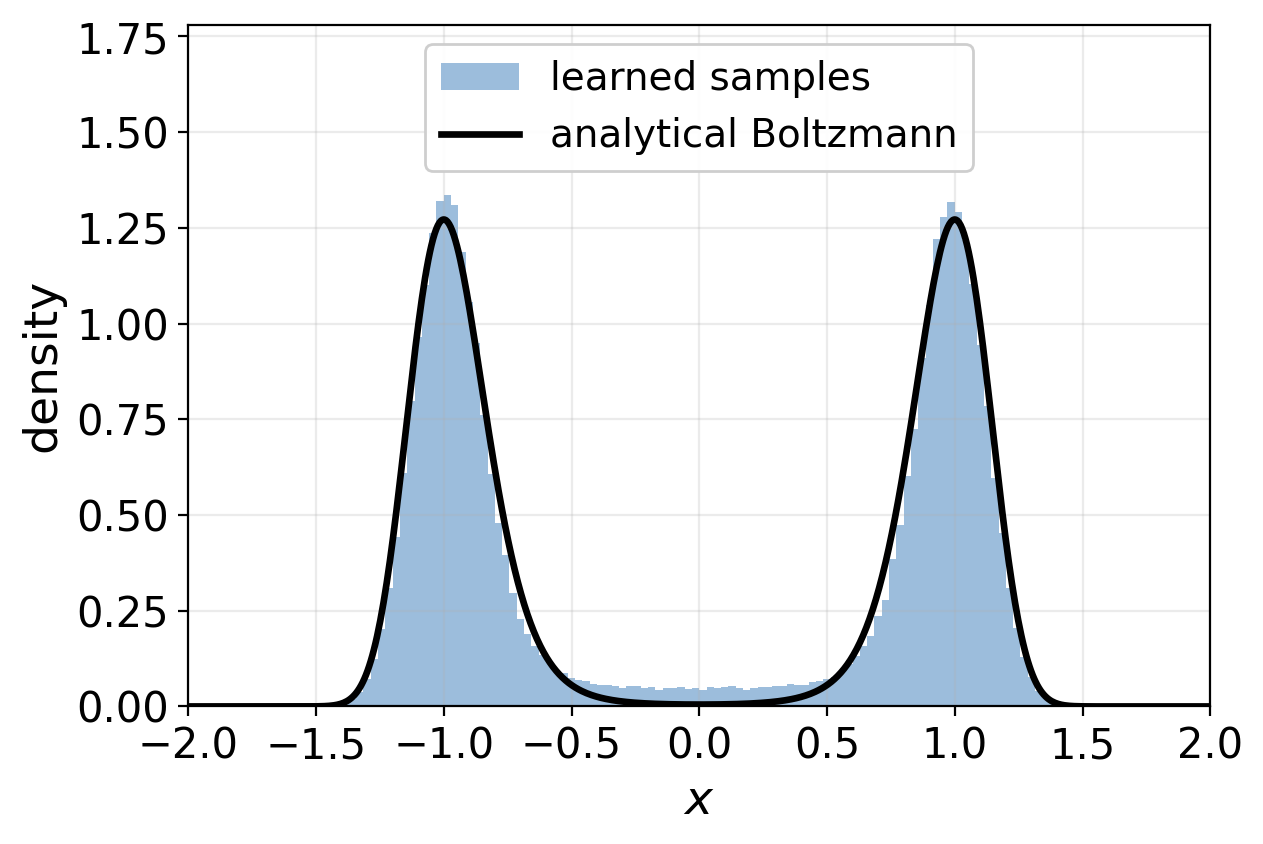
\includegraphics[width=\textwidth]{imgs/double_peak_muon_dist.png}
        \caption{}
    \end{subfigure}
    \hfill
    \begin{subfigure}[t]{0.455\textwidth}
        \centering
        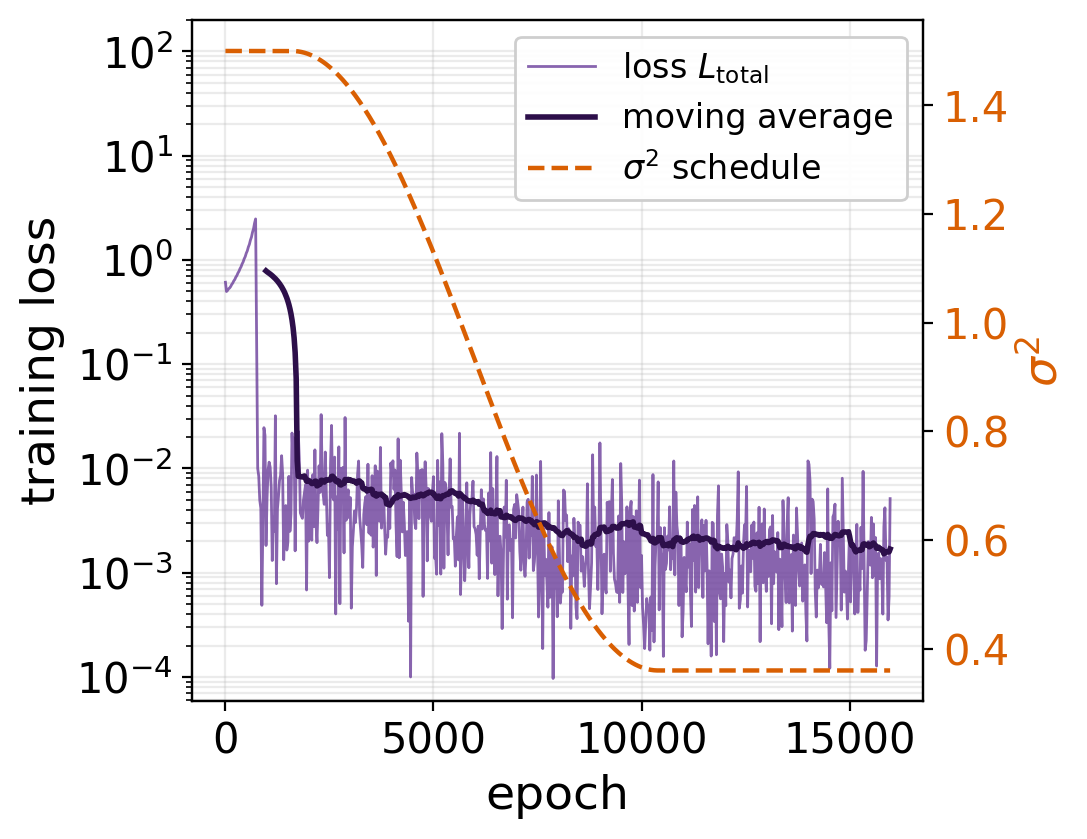
\includegraphics[width=\textwidth]{imgs/double_peak_muon_loss.png}
        \caption{}
    \end{subfigure}
    \caption{\revthree{Numerical results for the one-dimensional double-peak Fokker--Planck equation. (a) Learned distribution ($2\times 10^{5}$ samples) against the analytical Boltzmann density $\rho_{\text{true}} \propto \exp(-2V/\sigma^2)$. (b) Training loss ${L}_{\text{total}}$ (thin line: per-epoch value; thick line: moving average over $1{,}000$ epochs), together with the $\sigma^2$ annealing schedule on the right-hand axis. For the run shown, the Hellinger distance between the learned and analytical distributions is $0.091$ and the total-variation distance is $0.055$; the peak density exceeds the analytical value by $6\%$; the empirical standard deviation is $0.955$ against the exact value $0.972$; and the two wells carry $49.7\%$ and $50.3\%$ of the probability mass.}}
    \label{fig:double_peak}
\end{figure}

\revthree{The training loss decreases by more than three orders of magnitude, from $6.1 \times 10^{-1}$ at the start of training to $3.7 \times 10^{-4}$ at its end, with the decrease tracking the annealing of $\sigma^2$ (Figure~\ref{fig:double_peak}(b)). The neural pushforward mapping transforms the eight-dimensional Gaussian base samples into the target bimodal distribution, with peaks at $x \approx \pm 1$ in close agreement with the analytical Boltzmann density and with the mass split evenly between the two wells (Figure~\ref{fig:double_peak}(a)). Over three random seeds the Hellinger distance between the learned and analytical distributions is $0.110 \pm 0.025$. The residual discrepancy is concentrated near the transition state $x = 0$, where the learned density retains roughly $3.4$ times the analytical probability mass. This over-representation of the barrier region is a limitation of the method, discussed further in the Conclusion of the manuscript. An asymmetric variant of this problem is treated in \S4.1 of the manuscript.}

\FloatBarrier
\section{A two-dimensional double-peak problem}\label{sup:dp2d}

We extend the framework to a two-dimensional problem with two distinct probability peaks.

\subsection{Problem specification}
We consider the steady-state Fokker--Planck equation on $\mathbb{R}^2$ with dimension $n=2$, drift coefficient $\mathbf{b}(\mathbf{x}) = -\nabla V(\mathbf{x})$ where $V(x_1, x_2) = [(x_1-1)^2 + (x_2-1)^2][(x_1+1)^2 + (x_2+1)^2]$, and isotropic constant diffusion \revtwo{$a_{ij}(\mathbf{x}) = \sigma^2 \delta_{ij}$}.

The potential function $V(\mathbf{x})$ creates a double-well landscape with minima located at $(-1, -1)$ and $(1, 1)$. The drift is computed as:
\begin{align*}
b_1(\mathbf{x}) &= -2(x_1-1)[(x_1+1)^2 + (x_2+1)^2] - 2(x_1+1)[(x_1-1)^2 + (x_2-1)^2], \\
b_2(\mathbf{x}) &= -2(x_2-1)[(x_1+1)^2 + (x_2+1)^2] - 2(x_2+1)[(x_1-1)^2 + (x_2-1)^2].
\end{align*}

For this test, we set $\sigma = 0.4$. The analytical steady-state solution follows the Boltzmann distribution:
\begin{equation} \label{dp2d-rho-true}
\rho_{\text{true}}(\mathbf{x}) \propto \exp\left(-\frac{2V(\mathbf{x})}{\sigma^2}\right),
\end{equation}
which exhibits two prominent peaks centered at the potential minima.

\subsection{Training configuration}
The neural pushforward mapping $F_{\boldsymbol{\vartheta}}$ was implemented as a compact fully connected network with layer sizes $(16, 32, 32, 2)$, using Tanh activation functions. The input dimension of 16 provides a higher-dimensional base space to facilitate better mixing and exploration during training. The base distribution $\pi_{\text{base}}$ was chosen as a 16-dimensional standard Gaussian, i.e., $\mathbf{r} \sim \mathcal{N}(\mathbf{0}, \mathbf{I}_{16})$.

\revthree{The adversarial test functions form a mixed bank (\S2.2 of the manuscript) of $K=200$ plane waves $f^{(k)}(\mathbf{x}) = \varphi(\mathbf{w}^{(k)} \cdot \mathbf{x} + b^{(k)})$, for which $\mathcal{L}f$ is given by the general plane-wave form of \S2.2 of the manuscript. The bank consists of five families. The first contains $120$ plane waves with the sinusoidal envelope $\varphi = \sin$, initialized with $\mathbf{w}^{(k)} \sim \mathcal{N}(\mathbf{0}, \mathbf{I}_2)$ and $b^{(k)} \sim \mathcal{U}(0, 2\pi)$. The other four contain $20$ plane waves each, with the wavelet envelopes $\varphi(z) = e^{-z^2/2}$ (Gaussian), $\varphi(z) = (1-z^2)e^{-z^2/2}$ (Mexican hat), $\varphi(z) = 1-\tanh^2(z)$ (logistic) and $\varphi(z) = z\,e^{-z^2/2}$ (odd Hermite type). These $80$ wavelet-envelope functions are initialized with $|\mathbf{w}| \sim 4\cdot\mathcal{U}(0.5,1.5)$, a uniformly random direction, and offset $-b/|\mathbf{w}| \sim \mathcal{U}(-2,2)$, so that they cover both wells and the region between them. The five families are trained jointly by the adversary.} Both the test function parameters and the pushforward network were trained using their respective optimizers: stochastic gradient descent with learning rate $10^{-2}$ for the test functions, and Adam optimizer with learning rate $10^{-2}$ for the generator network. The batch size was set to $M=1{,}000$ samples.

The model was trained for \revthree{20,000} epochs. During training, the test functions were updated adversarially, with 5 gradient ascent steps \revthree{on the test-function parameters every 10 epochs}. This asymmetric update schedule helps maintain balance in the adversarial dynamics while ensuring the test functions remain sufficiently expressive to detect violations of the weak form.

\revthree{The relative barrier height of this potential, $2V(\mathbf{0})/\sigma^2 = 8/0.16 = 50$, is considerably larger than that of the one-dimensional example of \S\ref{sup:dp1d}. As in that example, we employ the $\sigma$-annealing curriculum of \S2.3 of the manuscript: $\sigma^2$ is held at $1.5$ for the first $10\%$ of the epochs, reduced to its target value $0.16$ along a cosine schedule over the following $55\%$, and held at $0.16$ thereafter.}

\subsection{Results and performance}

\begin{figure}[htb]
    \centering
    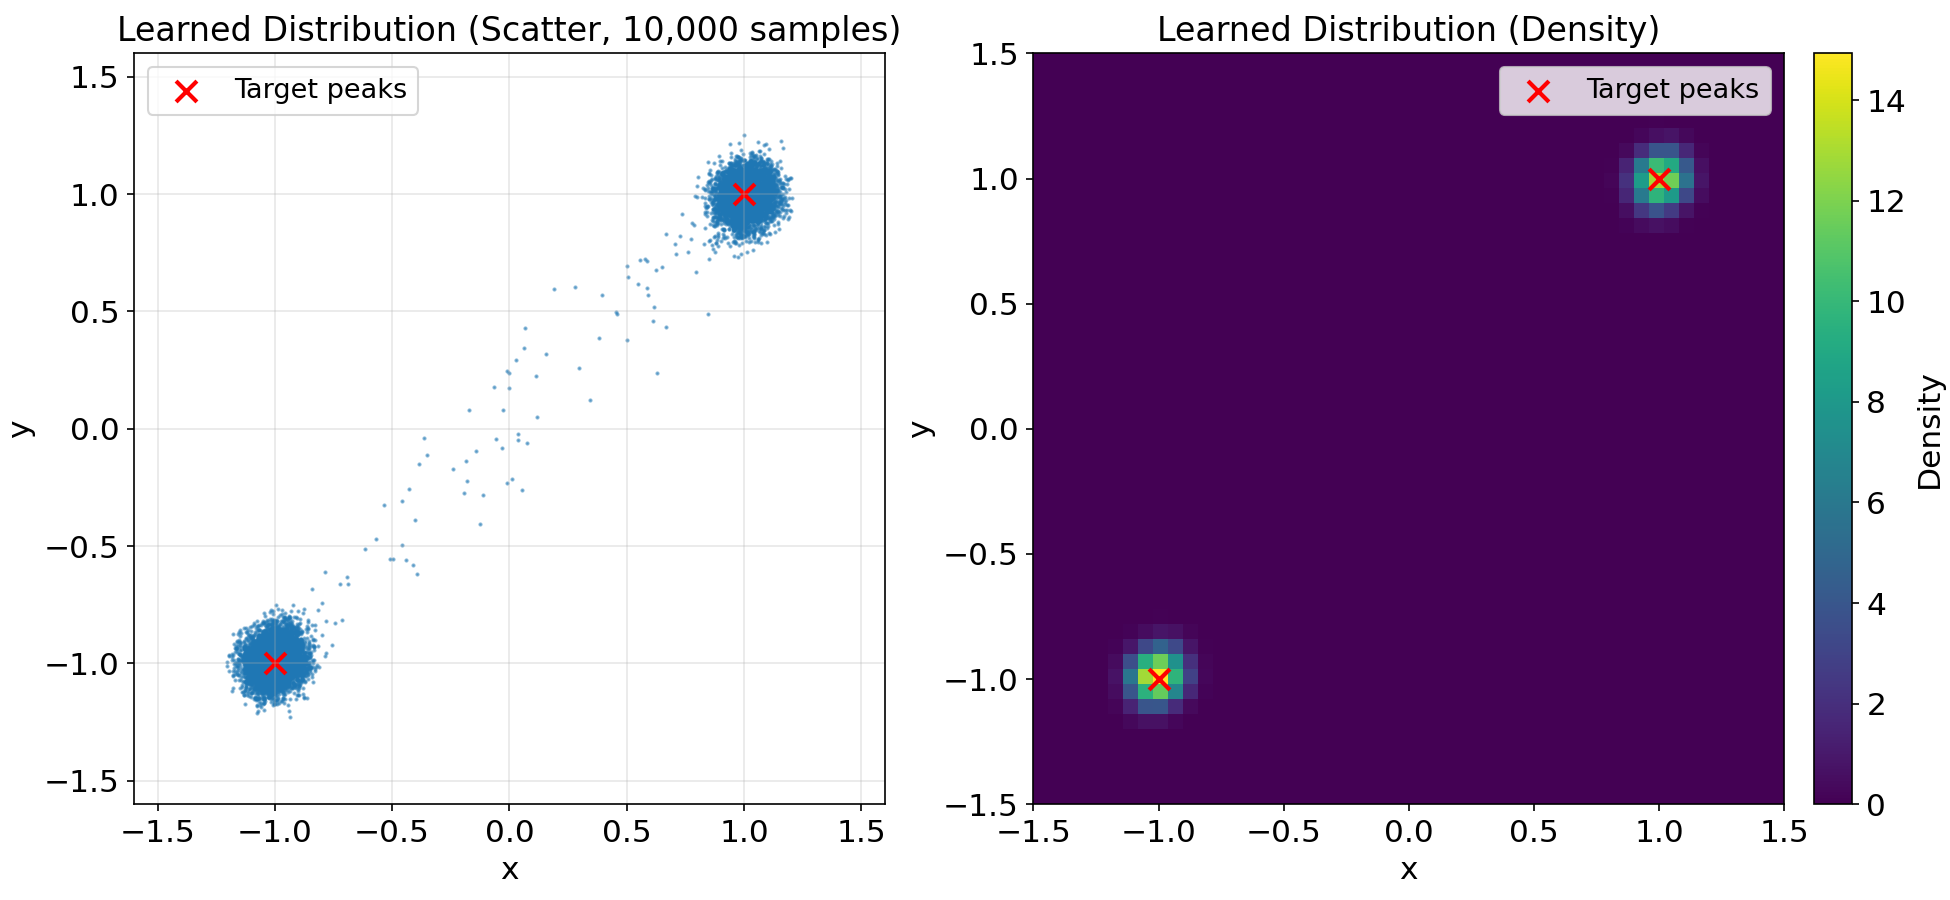
\includegraphics[width=0.7\textwidth]{imgs/double_peak_2d_plot1.png}
    \caption{Training results for the two-dimensional double-peak Fokker--Planck equation. Left: Scatter plot of \revthree{$10{,}000$} samples generated by the learned pushforward map, showing clear clustering at the target peaks $(-1,-1)$ and $(1,1)$ (marked with red crosses)\revthree{, together with a small number of samples scattered along the diagonal between them}. Right: Density heatmap \revthree{(from $2\times10^5$ samples)} revealing two distinct high-probability regions at the correct locations.}
    \label{fig:2d_result_training}
\end{figure}

\begin{figure}[htb]
    \centering
    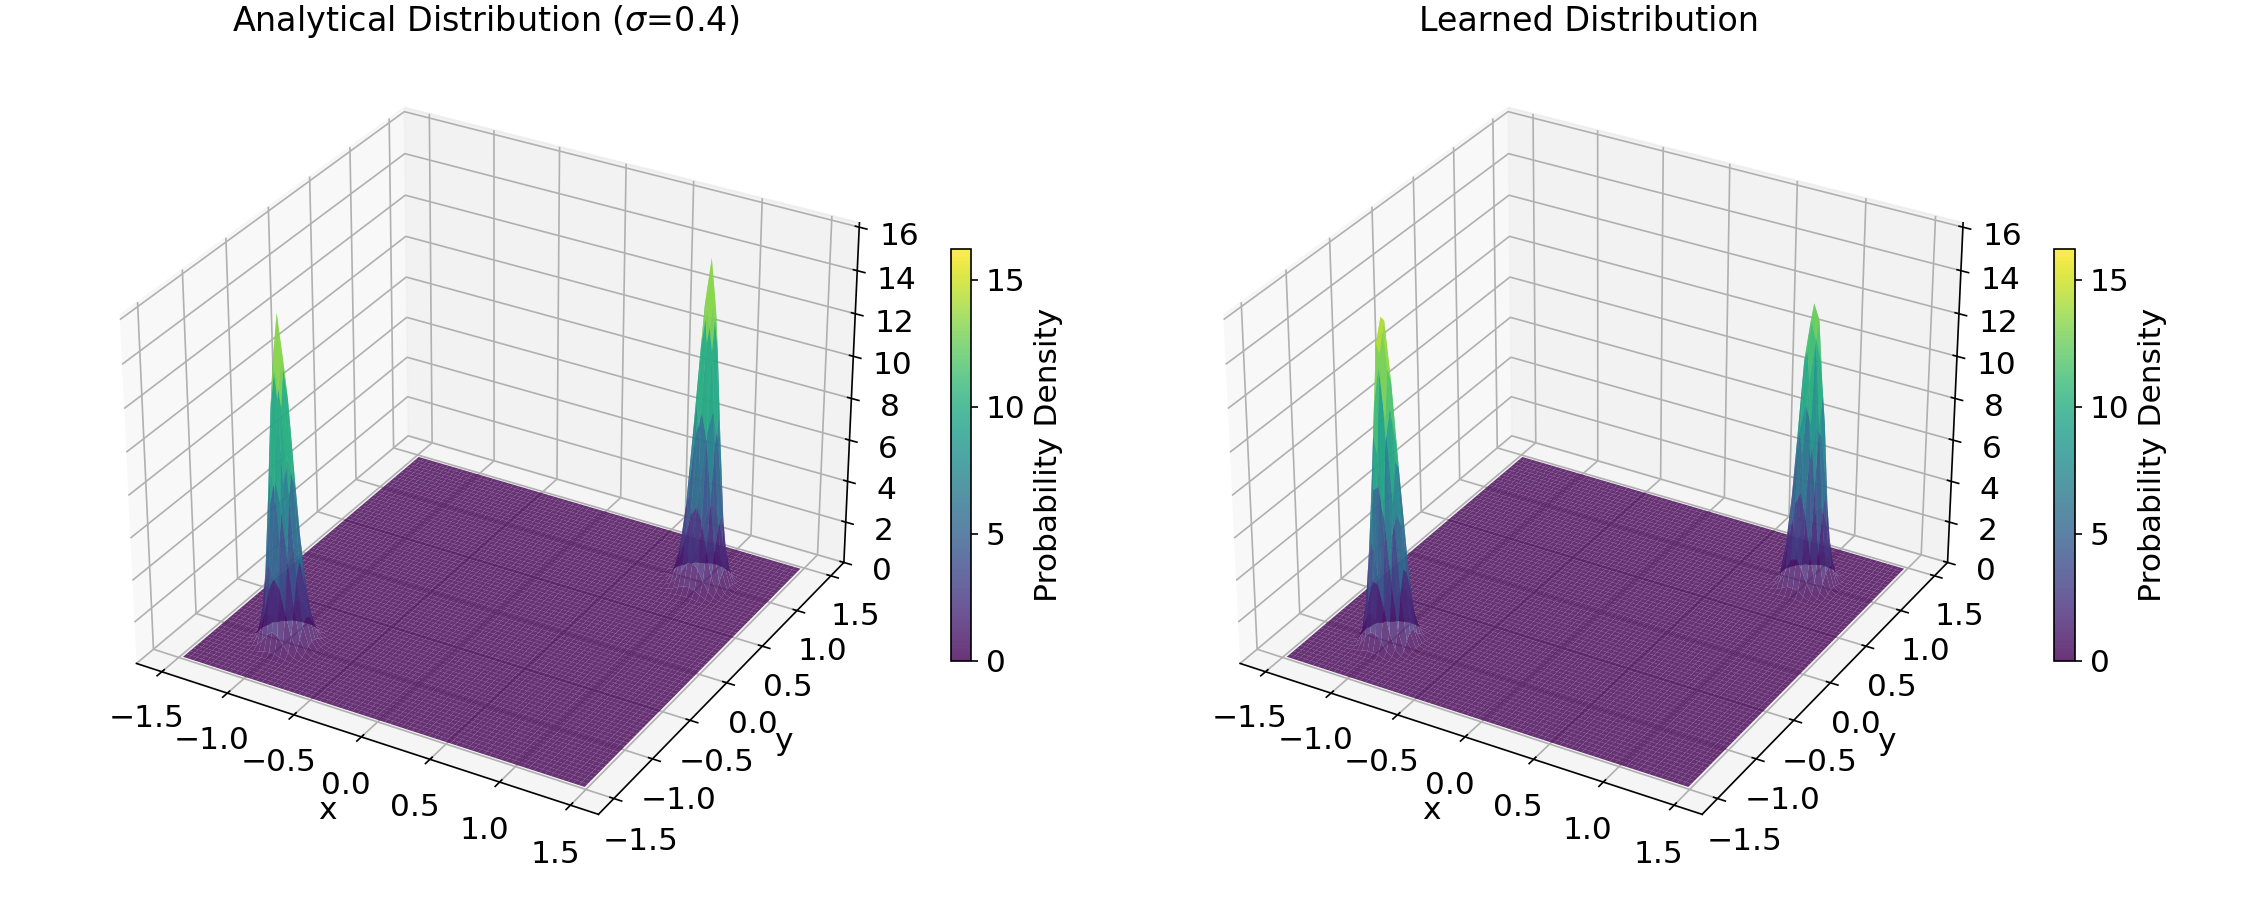
\includegraphics[width=\textwidth]{imgs/double_peak_2d_plot2.png}
    \caption{Comparison of analytical and learned probability distributions for the 2D double-peak problem. Left: Analytical Boltzmann distribution $\rho_{\text{true}}(\mathbf{x}) \propto \exp(-2V(\mathbf{x})/\sigma^2)$ with $\sigma=0.4$. Right: Learned distribution obtained from the pushforward network \revthree{($2\times10^5$ samples; both panels use the same $75\times75$ grid of cells)}. The two distributions show \revthree{close} agreement in both peak locations and overall shape.}
    \label{fig:2d_result_comparison}
\end{figure}

The training converged to a solution that captures the double-peak structure. As shown in Figure~\ref{fig:2d_result_training}, the scatter plot reveals clear bimodal clustering at the target positions $(-1, -1)$ and $(1, 1)$, with the density heatmap confirming probability concentration at these peaks.

Figure~\ref{fig:2d_result_comparison} shows \revthree{close} agreement between the analytical and learned distributions, with peaks at the correct locations and comparable peak heights and shapes. \revthree{For the run shown, the Hellinger distance between the learned and analytical distributions is $0.107$ and the total-variation distance is $0.084$ (both evaluated on a $120\times120$ grid over $[-2.5,2.5]^2$); the learned peak density is $1\%$ below the analytical value on the grid of Figure~\ref{fig:2d_result_comparison}; each learned well has standard deviation $0.072$ along the diagonal $x_1=x_2$ and $0.065$ across it, against the exact values $0.072$ and $0.071$; and the two wells carry $47.0\%$ and $53.0\%$ of the probability mass, against the exact even split. The training loss decreases from $7.2$ at the first epoch to $6.6\times10^{-3}$ (mean over the last $500$ epochs), following the annealing of $\sigma^2$.}

\revthree{A small fraction of the generated samples lies away from both wells, as can be seen in the left panel of Figure~\ref{fig:2d_result_training}. In the run shown, $0.75\%$ of the samples are farther than $0.35$ (about five standard deviations of a well) from both minima, whereas the analytical density assigns a probability of about $3\times10^{-5}$ to this region; these samples are spread thinly along the diagonal joining the two wells. Over three random seeds this fraction lies between $0.75\%$ and $2.2\%$, the Hellinger distance between $0.107$ and $0.136$, and the mass of the upper-right well between $47.0\%$ and $53.1\%$. We do not have a complete explanation for these residual samples. Two features of the method may contribute. First, $F_{\boldsymbol{\vartheta}}$ is continuous and the base distribution has connected support, so the support of the learned distribution is connected and cannot separate exactly into two components. Second, the drift vanishes at the saddle point $\mathbf{x}=\mathbf{0}$, so probability mass placed near it enters the weak-form residual only through the diffusion term, which is small at $\sigma=0.4$, and is therefore only weakly penalized by the loss.}

\revthree{Of the two ingredients of this training configuration---the $\sigma$-annealing curriculum and the mixed test-function bank---the curriculum has the larger effect on these samples: with the same settings but $\sigma^2$ fixed at $0.16$ throughout, the samples fail to concentrate at the wells within the $20{,}000$ epochs (between $44\%$ and $100\%$ of them lie away from both wells, over three seeds). The mixed test-function bank mainly improves the accuracy of the wells themselves: with the plane-wave functions alone ($K=200$, same curriculum) the Hellinger distance lies between $0.125$ and $0.227$ over three seeds, while the fraction of samples away from the wells, $0.8\%$ to $1.6\%$, is about the same as with the mixed bank. The curriculum thus reduces the residual samples substantially, but neither ingredient eliminates them.}

\end{document}
